\section{Wykorzystywane algorytmy}
\label{ref:Algorytmy}
W sekcji zostanie przybliżone działanie algorytmów (Rysunek \ref{fig:typy}) z uwzględnieniem znaczenia parametrów dobranych przez MetaOD.
Wszystkie algorytmy implementowane są z wykorzystaniem biblioteki \textit{Python Outlier Detection} (PyOD) \cite{zhao2019pyod}
\begin{figure}
    \centering
    \includegraphics[width=\textwidth]{chapters/istniejace/images/TypyAlgorytmów(1).png}
    \caption{Wykorzystywane algorytmy z podziałem na metodologię.}
    \footnotesize{źródło: Opracowanie własne}
    \label{fig:typy}
\end{figure}

\subsection{OCSVM}
\textit{One-Class SVM} [Jednoklasowa maszyna wektorów nośnych] (OCSVM) \cite{ocsvm}. OCSVM jest binarną metodą klasyfikacji odwzorowującą dane wejściowe z wykorzystaniem funkcji jądrowej na wielowymiarową w poszukiwaniu hiperpłaszczyzny separującej poprawne obserwacje od anomalii.  
% Model jądrowy:
% \begin{equation}
%     f(x) = \sum_{i=1}^{N} \alpha _i y_iK(x_i,x)+b
% \end{equation}
% gdzie $K$ jest funkcją jądrową:
Funkcje jądrowe:
\begin{align*}
    Liniowa: x^Tx_i \\
    Wielomianowa: (\gamma x^Tx_i+c)^n \\
    RBF: exp(-\gamma ||x-x_i||^2) \\
    Sigmoidalna: tgh(\gammax^Tx_i+c)
\end{align*}
Parametr "nu" jest górną granicą akceptowalnego błędu klasyfikacji oraz dolną granicą liczby wektorów nośnych do liczby analizowanych obserwacji. Wykorzystany w celu uniknięcia przeuczenia klasyfikatora. 
\label{eq:funjadro}

\subsection{kNN}
\label{knn}
\textit{k-Nearest Neighbors}[Algorytm k najbliższych sąsiadów] (kNN) \cite{knn} opiera się na wnioskowaniu, że poprawne obserwacje będą w sąsiedztwie innych poprawnych obserwacji. Natomiast anomalie będą znacząco oddalone od skupień normalnych obserwacji. Dla każdego elementu obliczamy metrykę do k = 1,...,N sąsiada. Wynik anomalności elementu zależy od metody (wybrana przez MetaOD):
\begin{itemize}
    \item \textit{largest} - anomalność punktu jest odległością do k-sąsiada (najdalej oddalonego)
    \item \textit{mean} - anomalność punktu jest średnią ze wszystkich odległości do sąsiadów
    \item \textit{median} - anomalność punktu jest medianą wszystkich odległości do sąsiadów
\end{itemize}

\subsection{LOF}
\label{lof}
\textit{Local Outlier Factor} (LOF) \cite{lof} algorytm w odróżnieniu od algorytmu kNN rozpatruje lokalną gęstość względem sąsiadów. Podejście odnosi się do wad metod opartych na metryce w przypadkach zbiorów danych o różnych gęstościach klastrów poprawnych obserwacji (Rysunek \ref{fig:anomalie_glob_lok}).
W celu obliczenia anomalności punktu należy dokonać 3 kroków:
\begin{enumerate}
    \item Dla rozpatrywanego punktu x, należy znaleźć k najbliższych sąsiadów
    \item Rozpatrując k najbliższych sąsiadów $N_k$, wyznaczyć zagęszczenie w k-sąsiedztwie punktu x obliczając \textit{local reachability density}(LRD): 
    \begin{equation}
        LRD_k(x) = 1/\Bigg(\frac{ \sum\limits_{o \in N_k(x)} d_k(x,o) }{|N_k(x)|}\Bigg)
    \end{equation}
    gdzie $d_k(\cdot)$ oznacza \textit{reachability distance}
    \item Ostatecznie obliczamy wartość LOF, porównując LRD punktu $x$ z LRD k-sąsiada:
    \begin{equation}
        LOF(x) = \frac{ \sum\limits_{o \in N_k(x)} \frac{LRD_k(o)}{LRD_k(x)} }{|N_k(x)|}
    \end{equation}
\end{enumerate}
Wynik LOF jest stosunkiem LRD punku x do średniej LRD dla k sąsiadów.
% współczynnikiem lokalnej gęstości.
Jeżeli wartość $LOF(x)>1$ oznacza to małą lokalną gęstość (anomalia lokalna). 
$LOF(x) \approx 1$ oznacza, że lokalna gęstość punktu x jest zbliżona do sąsiadów.

\subsection{COF}
\label{cof}
\textit{Connectivity based Outlier Factor}(COF) \cite{cof} algorytm COF jest zbliżony działaniem do LOF, główną różnicą wybór k najbliższych sąsiadów (Rysunek \ref{fig:lcof}). LOF wybiera k najbliższych sąsiadów, wykorzystując metrykę np. odległość euklidesową, tworząc wokół analizowanego punktu sferę. COF tworzy zbiór k-sąsiadów dla punktu x, wybierając najbliższego sąsiada, którego dodaje do zbioru. Następnie wybiera punkt najbliższy do dowolnego elementu istniejącego zbioru k-sąsiadów i dodaje go do zbioru. Proces przebiega do momentu, aż zbiór zawierać będzie k elementów. Wynikiem czego powstaje minimalne drzewo rozpinające. Odpowiednikiem \textit{reachability distance} jest \textit{chaining distance} czyli długość krawędzi w minimalnym drzewie rozpinającym..
Obliczanie anomalności punktu x jest analogiczne do LOF -- stosunek \textit{chaining distance} dla punktu x do średniej z \textit{chaining distance} dla k-sąsiadów :
\begin{equation}
    COF_k(x) = \frac{|N_k(x)| \cdot ac-dist_{N_K(x)}(x)}{\sum\limits_{o \in N_k(x)}ac-dist_{N_k(o))}(o)}
\end{equation}
gdzie $ac_{dist}(x)$ oznacza średnią długość krawędzi w minimalnym drzewie rozpinającym punktu $x$

\begin{figure}
    \centering
    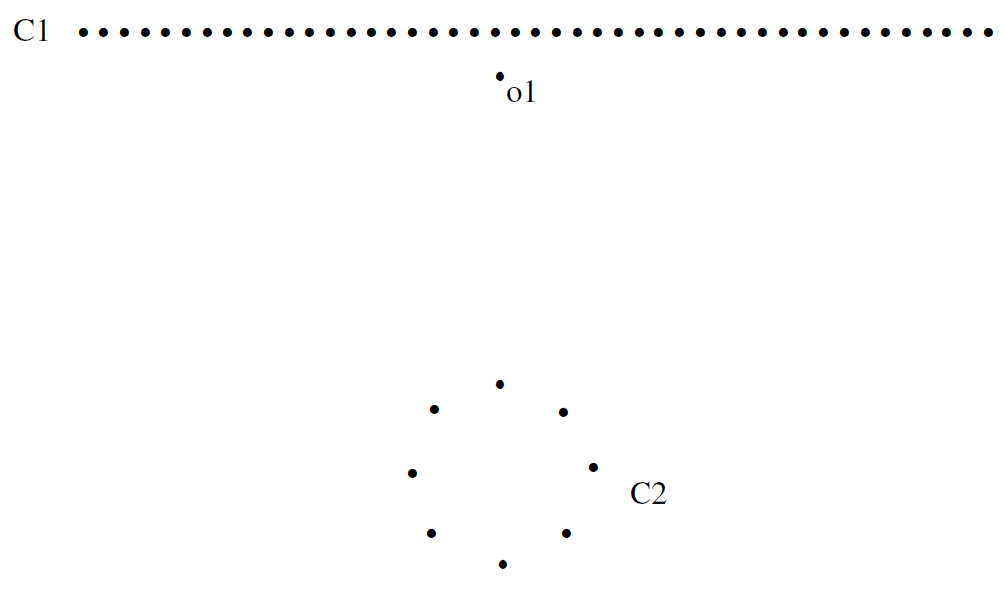
\includegraphics[width=.7\textwidth]{chapters/MetaOD/images/cof.png}
    \caption{Zbiór dla którego skuteczna detekcja anomalii algorytmem LOF nie powiedzie się.}
    \footnotesize{źródło: \cite{cof}}
    \label{fig:cof}
\end{figure}

\begin{figure}
    \centering
    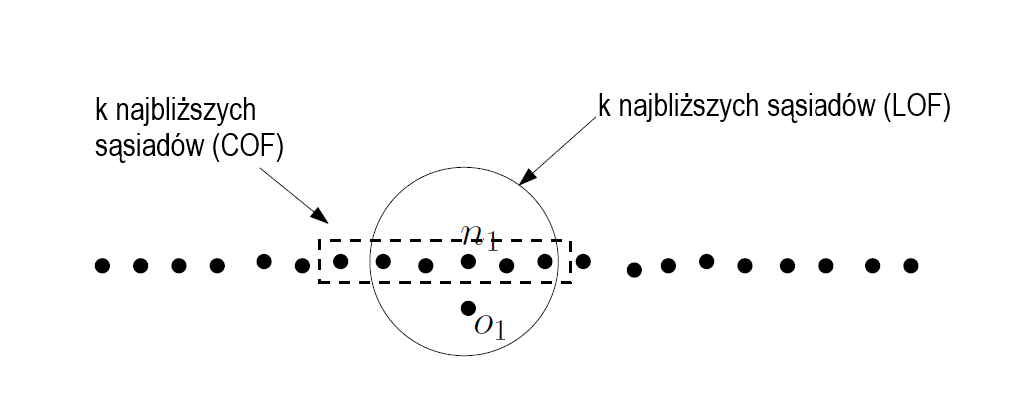
\includegraphics[width=.8\textwidth]{chapters/MetaOD/images/lvcof.png}
    \caption{Różnica w wyborze k najbliższych sąsiadów dla COF i LOF (k=5).}
    \footnotesize{źródło: Opracowanie własne na podstawie  \cite{chandola2009anomaly}}
    \label{fig:lcof}
\end{figure}

\subsection{ABOD}
\label{abod}
\textit{Angel-based Outlier Detection}(ABOD) \cite{abod} zamiast metryki między punktami w sąsiedztwie obserwacji, porównuje kierunek wektorów skierowanych wychodzących z rozpatrywanego punktu $x$.  W wielowymiarowych przestrzeniach kąty są stabilniejsze niż metryka, spowodowane jest to ,,przekleństwem wymiarowości''. Rezultatem badań na temat zagadnienia ,,przekleństwa wymiarowości"\cite{curse} jest wniosek, że najdalszy i najbliższy punkt wraz ze wzrostem wymiarów, zbiegają do 0 :
\begin{equation}
\lim_{d\to\infty} \frac{dist_{max} - dist_{min}}{dist_{min}} \longrightarrow 0
\end{equation}
Z tego powodu np. w grupowaniu dokumentów tekstowych jako miary podobieństwa wykorzystuje się miarę kosinusową \cite{huang2008similarity}. Algorytm ABOD rozpatruje wszystkie punkty w zbiorze w odniesieniu do analizowanego punktu, jest to podejście o wysokiej złożoności obliczeniowej $O(n^3)$. W celu zmniejszenia złożoności obliczeniowej w pracy wykorzystano FastABOD, który rozpatruje k-sąsiadów.

Rysunek \ref{fig:abod} obrazuje intuicję algorytmu ABOD, który do oceny anomalności punktu stosuje współczynnik \textit{Angle-based outlier factor}(ABOF):
\begin{equation}
    ABOF(x) = Var\frac{\langle \overrightarrow{xy}, \overrightarrow{xz} \rangle⟩}{\big\| \overrightarrow{xy\big\|}\big\| \overrightarrow{xz}\big\|},y,z \in B
\end{equation}
gdzie $B$ jest odpowiednio dobranym zbiorem, jako iż w pracy wykorzystano algorytm FastABOD, jest to zbiór k-sąsiadujących punktów. Im niższy ABOF tym większe podejrzenie anomalii
% (PyOD w celu zachowania konwencji -- większa wartość wyjściowa algorytmu oznacza wyższą anomalność obserwacji -- stosuje przeciwność ABOF tzn. -ABOF)
\begin{figure}
    \centering
    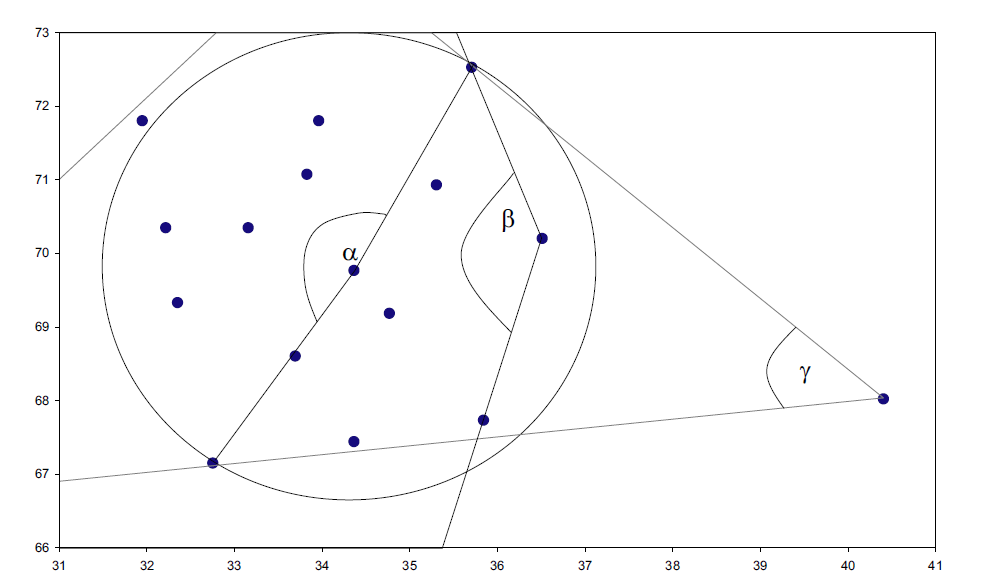
\includegraphics[width=.65\textwidth]{chapters/MetaOD/images/abod.png}
    \caption{Intuicja kierująca algorytmem ABOD.}
    \footnotesize{źródło: \cite{abod}}
    \label{fig:abod}
\end{figure}

\subsection{HBOS}
\textit{Histogram-based Outlier Score} (HBOS) \cite{hbos} 
zakłada niezależność cech. Określa anomalność punktu, budując histogramy o n prostokątach
dla każdej cechy. Częstotliwość obserwacji przypadających do każdego prostokąta histogramu tożsama jest z zagęszczeniem cechy. Następnie każdy histogram przechodzi normalizacje tak, aby maksymalna wysokość dla każdego histogramu wynosiła 1. Zapewnia to równą wagę każdego histogramu w procesie obliczania anomalności punktu (HBOS). Anomalność punktu x wyznacza się według wzoru:
\begin{equation}
    HBOS(x)= \sum\limits^d_{i=0}log(\frac{1}{hist_i(x)})
\end{equation}

\subsection{LODA}
\label{loda}
\textit{Lightweight Online Detector of Anomalies}(LODA) \cite{loda}
% wykorzystuje podejście budowania silnego klasyfikatora składającego się ze słabszych klasyfikatorów (zespół klasyfikatorów). Stosuje technikę losowych projekcji (\textit{Random projection}) w celu redukcji wymiaru \cite{raf2017}. 
wykorzystuje podejście budowania silnego klasyfikatora składającego się ze słabszych klasyfikatorów (zespół klasyfikatorów). Stosuje technikę losowych projekcji (\textit{Random projection}) w celu redukcji wymiaru, $\mathbb{R}^d \rightarrow \mathbb{R}^k$  \cite{raf2017}, gdzie $k$ dobrane przez MetaOD -- liczba losowych cięć.
% Tworzy $\{w_i \in \mathbb{R}^d \}^k_{i=1}$ niezerowych wektorów o wymiarze liczby cech analizowanego zbioru danych.
LODA składa się z k jednowymiarowych histogramów $\{h_i\}^k_{i=1}$ o liczbie prostokątów dobranym przez MetaOD oraz wektorów projekcji $\{w_i \in \mathbb{R}^d \}^k_{i=1}$. Każdy z histogramów przybliża gęstość zmiennej losowej (obserwacji) rzutowanej w kierunku wektora $w_i$. 
% Reszta elementów wektora generowana jest według rozkładu normalnego $N(0,1)$.
Wynik anomalności dla punktu x wyznacza się ze wzoru:
\begin{equation}
    f(x) = -\frac{1}{k}\sum\limits^k_{i=1}log\hat{p}_i(x^Tw_i)
\end{equation}
gdzie $\hat{p}$ oznacza gęstość zmiennej losowej przybliżonej przez i-ty histogram.
\subsection{IForest}
\label{iforest}
\label{sub:IF}
\textit{Isolation Forest}(IForest) \cite{iforest} wykorzystuje teorię drzew i lasów losowych. Izoluje obserwacje, wybierając losowo cechę i rozdziela ją na podstawie losowej wartości progowej (Rysunek \ref{fig:iforest}). W odróżnieniu od drzew decyzyjnych i losowych lasów, zamiast problemu klasyfikacji obliczana jest odległość między korzeniem a liściem (odizolowaną obserwacją). Krótsza odległość między korzeniem a liściem tym łatwiej odizolować obserwację na podstawie losowo wybranych cech. Uśredniona odległość pomiędzy wszystkie drzewa decyzyjne jest wartością anomalności obserwacji. Liczba estymatorów określa liczbę drzew decyzyjnych. Procent rozpatrywanych cech jest odsetkiem losowo wybranych cech wykorzystanych dla każdego estymatora.

\begin{figure}[h]
    \centering
    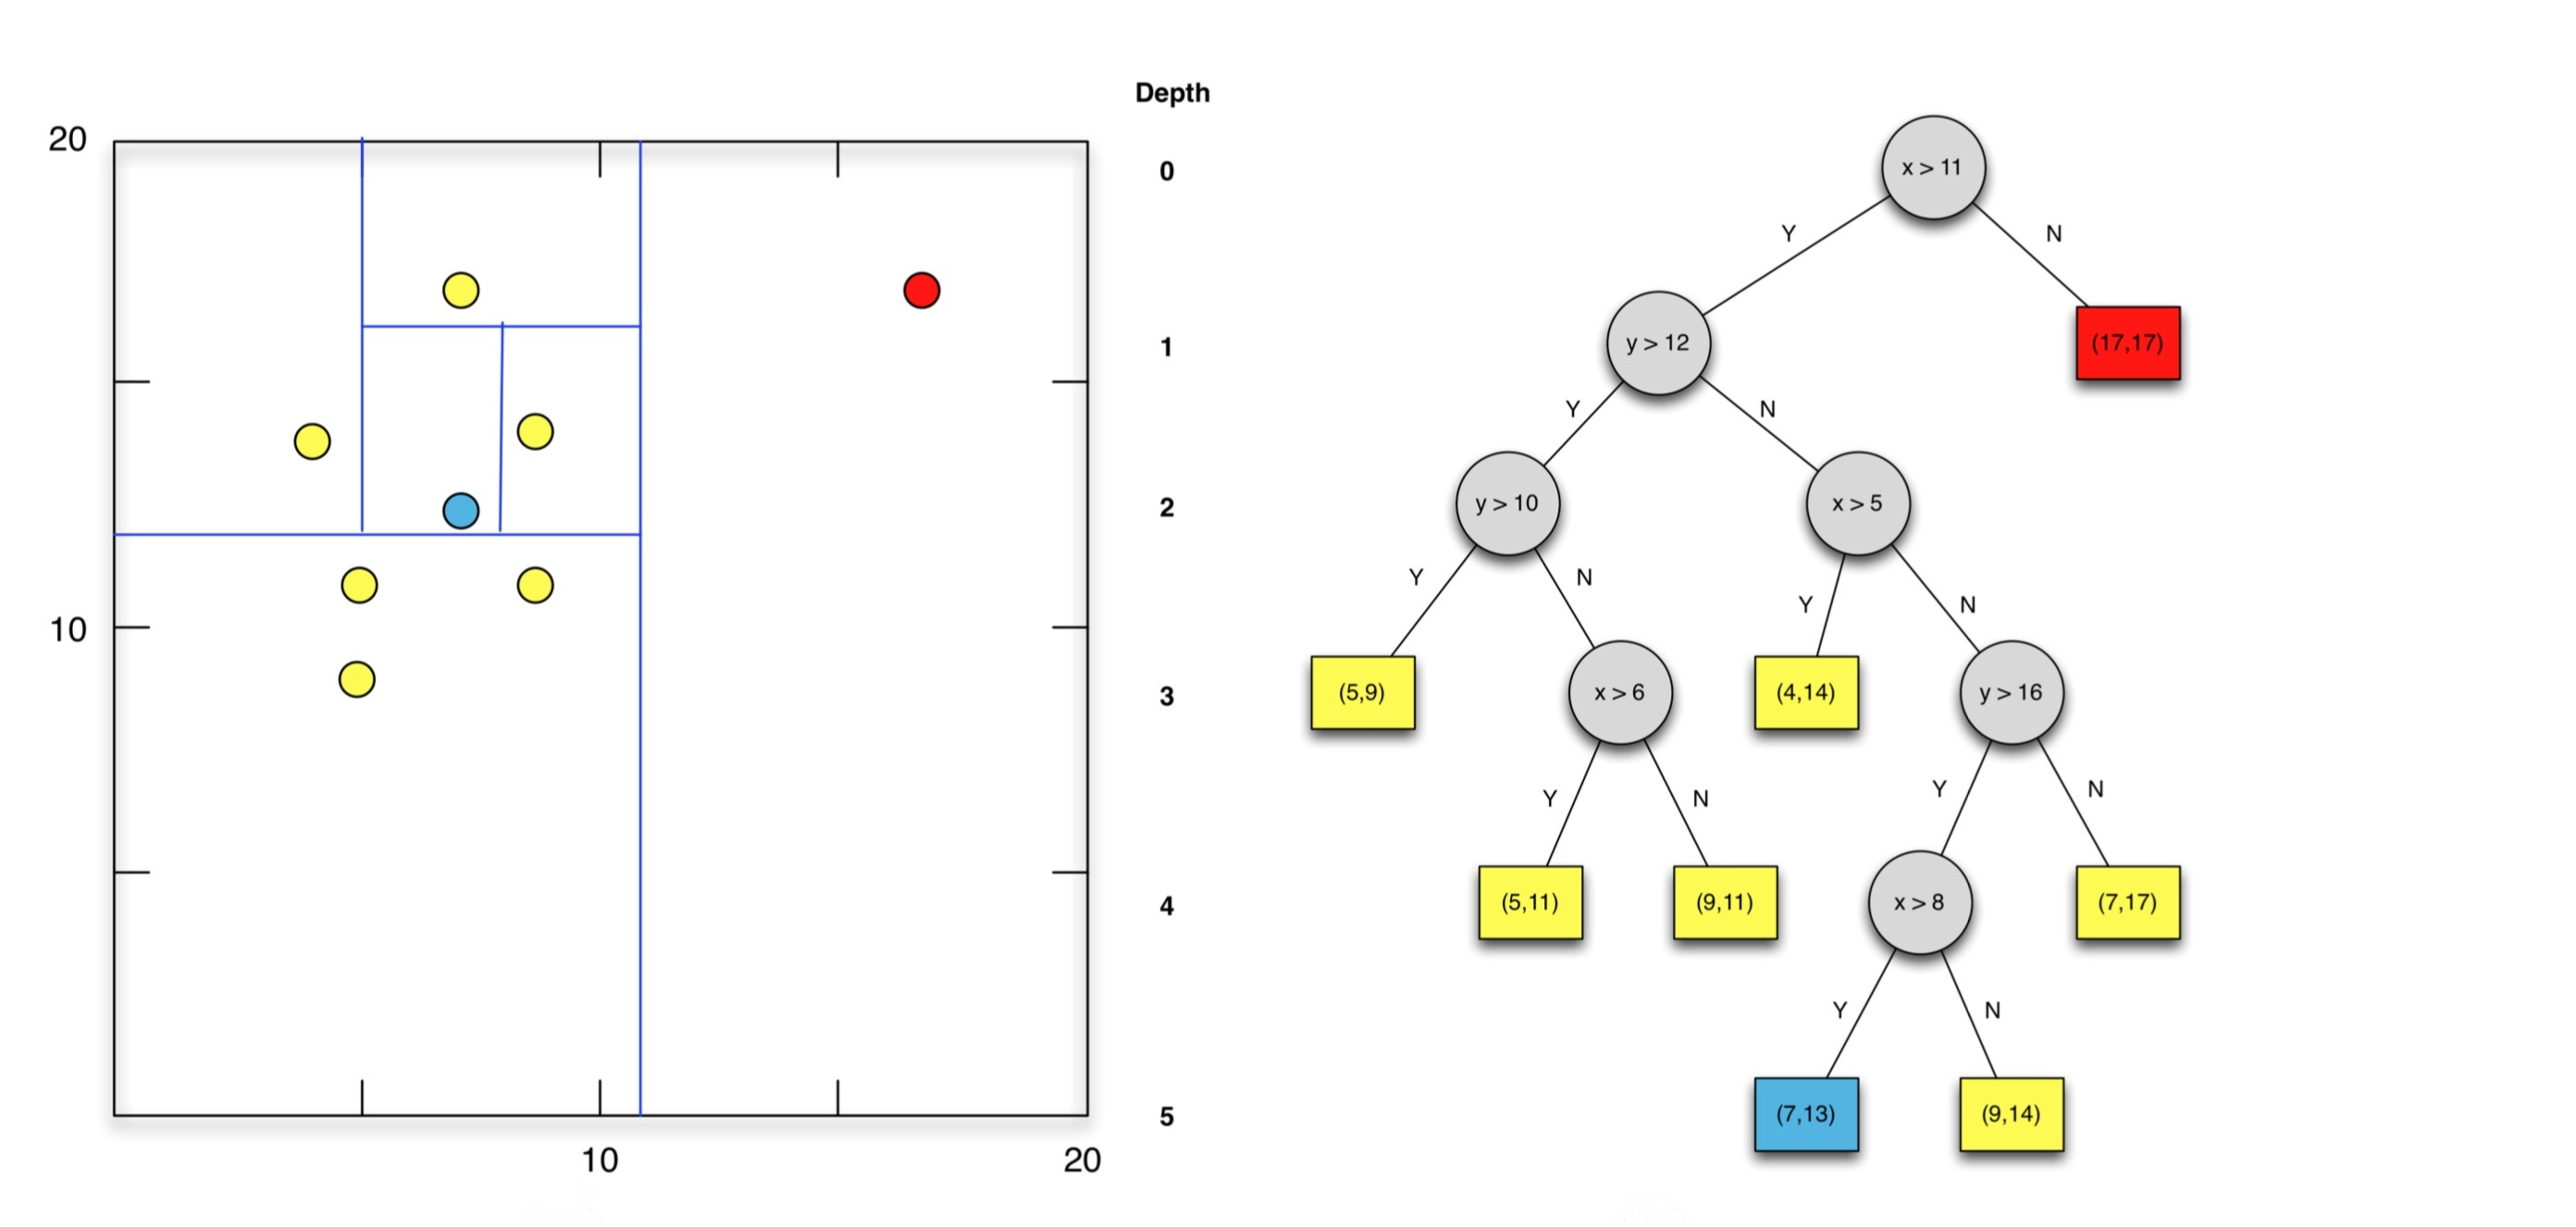
\includegraphics[width=.8\textwidth]{chapters/MetaOD/images/iforest.jpg}
    \caption{Drzewo decyzyjne w \textit{Isolation Forest}.}
    \footnotesize{źródło: \cite{if-image}}
    \label{fig:iforest}
\end{figure}

